\section{Pattern Classification on Linearly Separable Data}

% Subsection 1 - KNN Model -----------------------------------
\subsection{K-Nearest Neighbours Classifier}

The given synthetic data is classified using the KNN Method. The data is already well separated into classes. Thus a very good performance for even K=1 is observed. A 100$\%$ accuracy is observed in all training, validation and test set for all the tested values of K. The decision region is also plotted and the training data is overlapped with it. Let us look at some interesting plots obtained for the KNN method for the given dataset. \\

The decision plot for K=1 is shown in [\ref{fig:2}]. As can be observed, the decision boundary is slightly distorted for lower values of K. On the other hand, as the values of K increases we get a more smoother decision boundary as can be seen in [\ref{fig:6}] for K=15. 

% -----------------------------------------------------------

{\rowcolors{3}{green!40!yellow!10}{green!0!yellow!30}
\begin{table}[!h]
\centering
\begin{tabular}{ |c|c|c|  }
\hline
\rowcolor{lightgray} Model & Training Accuracy & Val Accuracy\\
\hline
K=1 & 100$\%$  & 100$\%$ \\   
 \hline
K=7 & 100$\%$  & 100$\%$ \\ 
 \hline
K=15 & 100$\%$  & 100$\%$ \\ 
\hline
\end{tabular}
\caption{Performance of various KNN Models}.
\label{table:1}
\end{table}
}

\newpage
% -----------------------------------------------------------
\subsubsection*{Plots for K=1}

\begin{figure}[!ht]
    \centering
    \begin{subfigure}[t]{0.5\textwidth}
        \centering
        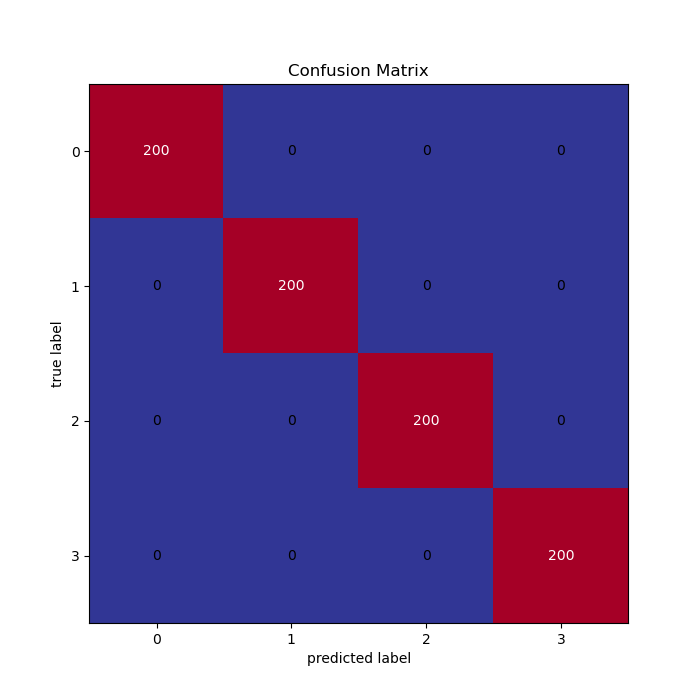
\includegraphics[height=2.5in]{Dataset_1a/K_1_cmatrix_train_data.png}
        \caption{Confusion Matrix for training data}
    \end{subfigure}%
    ~ 
    \begin{subfigure}[t]{0.5\textwidth}
        \centering
        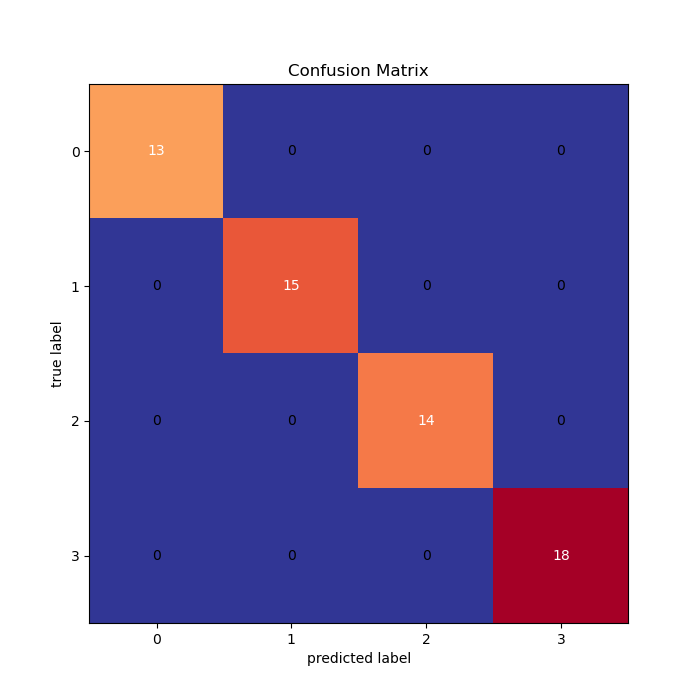
\includegraphics[height=2.5in]{Dataset_1a/K_1_cmatrix_test_data.png}
        \caption{Confusion Matrix for test data}
    \end{subfigure}%
    ~
    \caption{Confusion Matrix for KNN Model trained with K=7}
    \label{fig:1}
\end{figure}


% -----------------------------------------------------------
\begin{figure}[!ht]
    \centering
    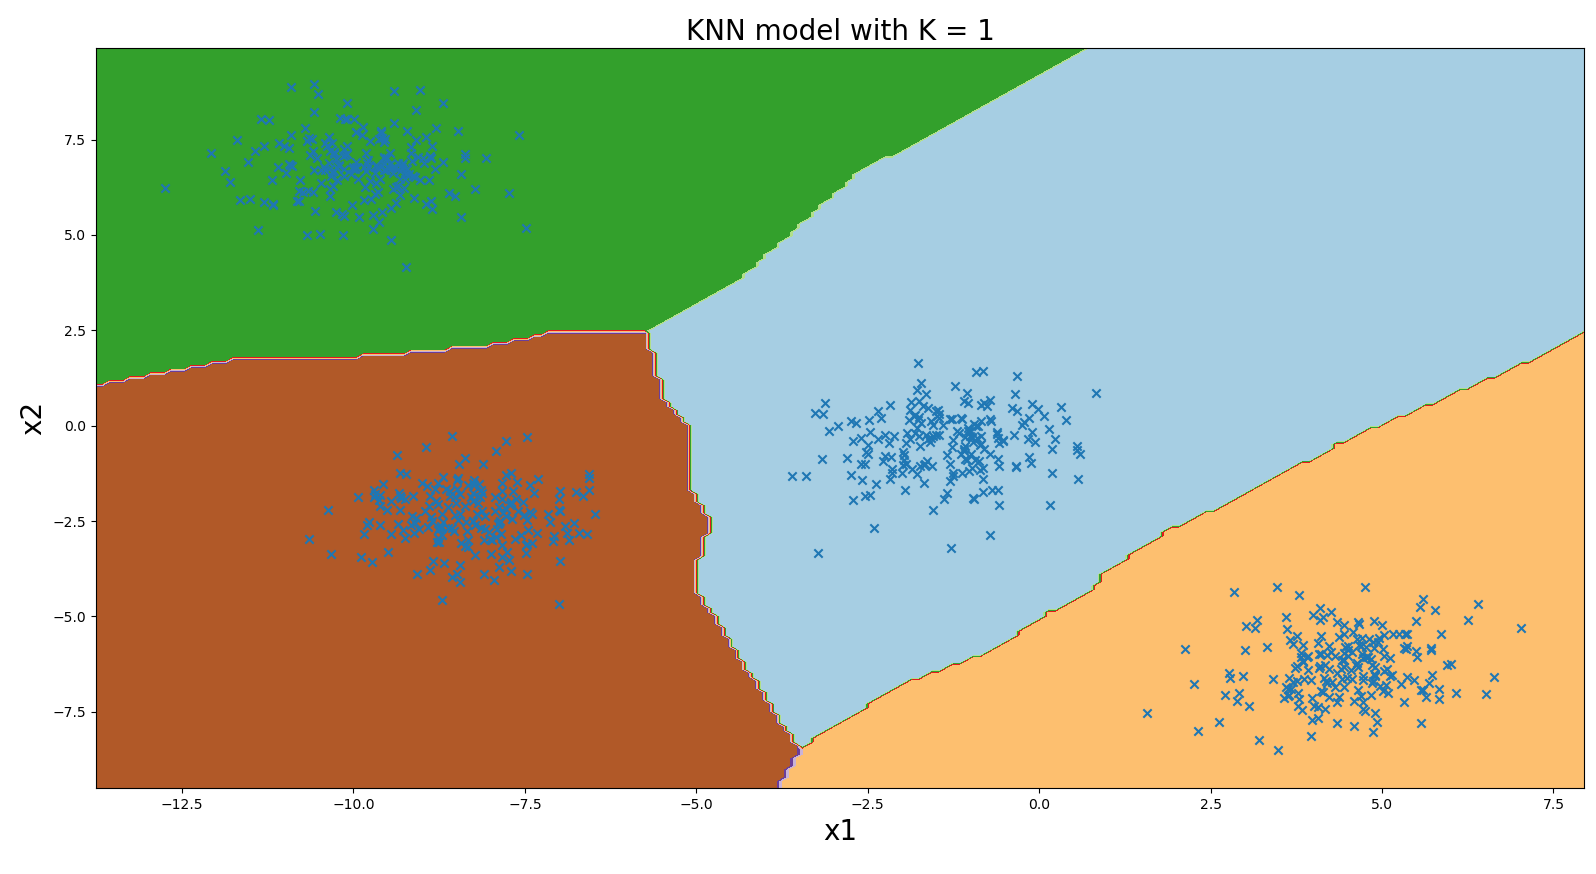
\includegraphics[height=3.5in,width=4in]{Dataset_1a/K_1_decision_plot.png}
    \caption{Decision Plot KNN Model trained with K=1}
    \label{fig:2}
\end{figure}

\newpage
% -----------------------------------------------------------
\subsubsection{Plots for K=7}

\begin{figure}[!ht]
    \centering
    \begin{subfigure}[t]{0.5\textwidth}
        \centering
        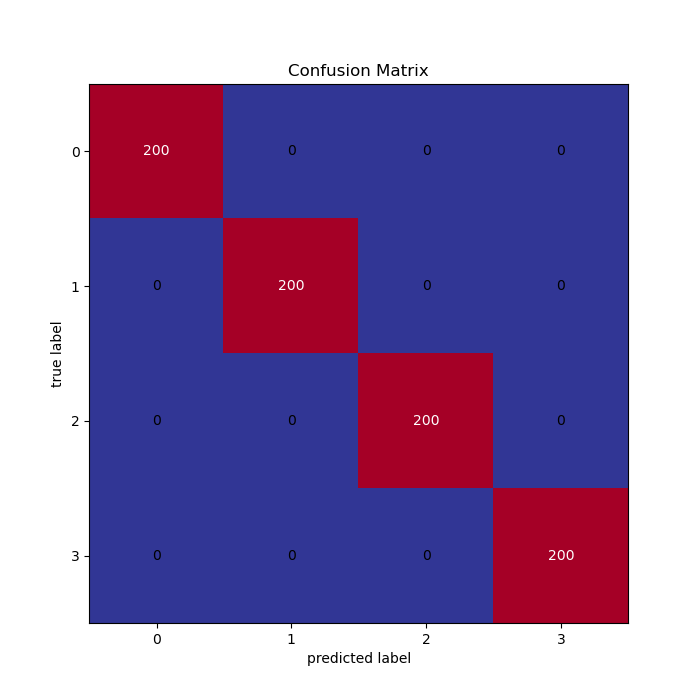
\includegraphics[height=2.5in]{Dataset_1a/K_7_cmatrix_train_data.png}
        \caption{Confusion Matrix for training data}
    \end{subfigure}%
    ~ 
    \begin{subfigure}[t]{0.5\textwidth}
        \centering
        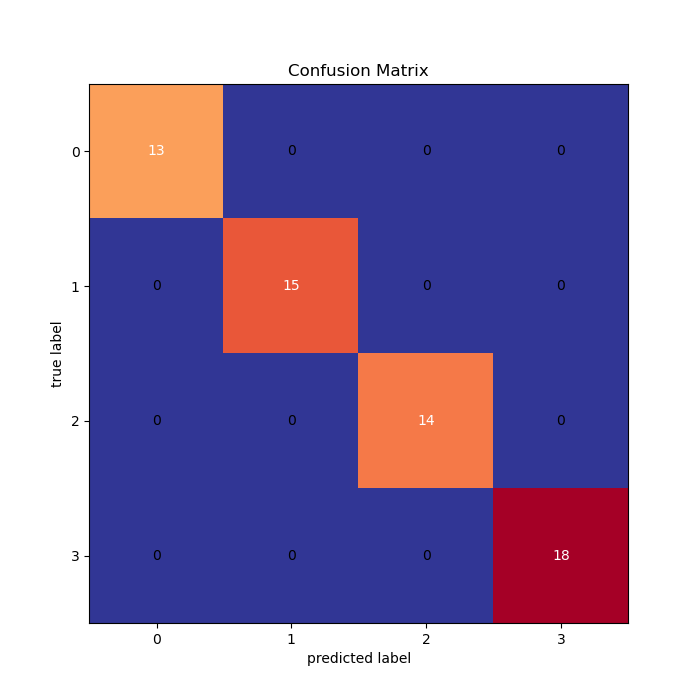
\includegraphics[height=2.5in]{Dataset_1a/K_7_cmatrix_test_data.png}
        \caption{Confusion Matrix for test data}
    \end{subfigure}%
    ~
    \caption{Confusion Matrix for KNN Model trained with K=7}
    \label{fig:3}
\end{figure}
% -----------------------------------------------------------
\begin{figure}[!ht]
    \centering
    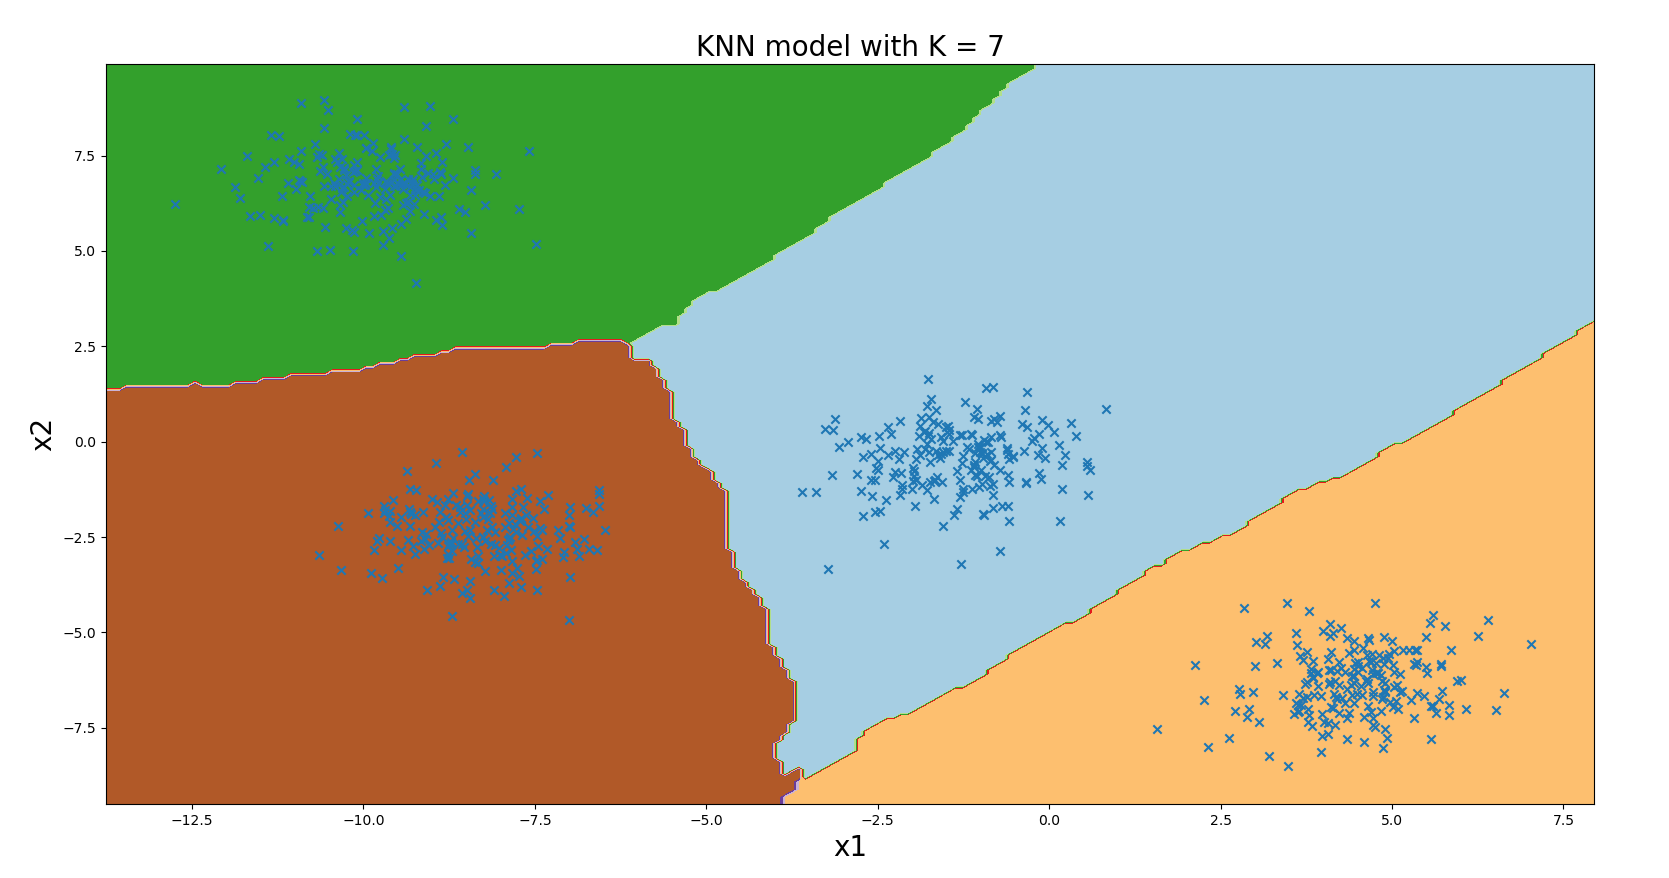
\includegraphics[height=3.5in,width=4in]{Dataset_1a/K_7_decision_plot.png}
    \caption{Decision Plot KNN Model trained with K=7}
    \label{fig:4}
\end{figure}

\newpage
% -----------------------------------------------------------
\subsubsection{Plots for K=15}

\begin{figure}[!ht]
    \centering
    \begin{subfigure}[t]{0.5\textwidth}
        \centering
        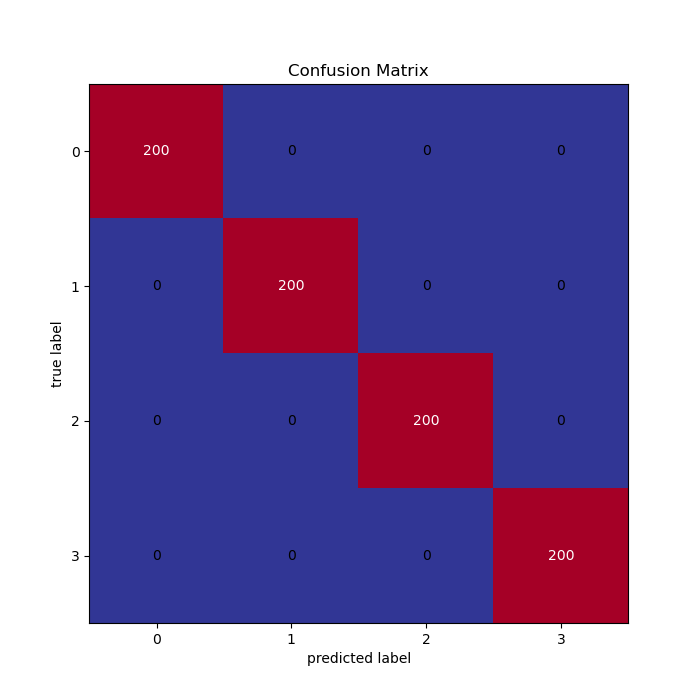
\includegraphics[height=2.5in]{Dataset_1a/K_15_cmatrix_train_data.png}
        \caption{Confusion Matrix for training data}
    \end{subfigure}%
    ~ 
    \begin{subfigure}[t]{0.5\textwidth}
        \centering
        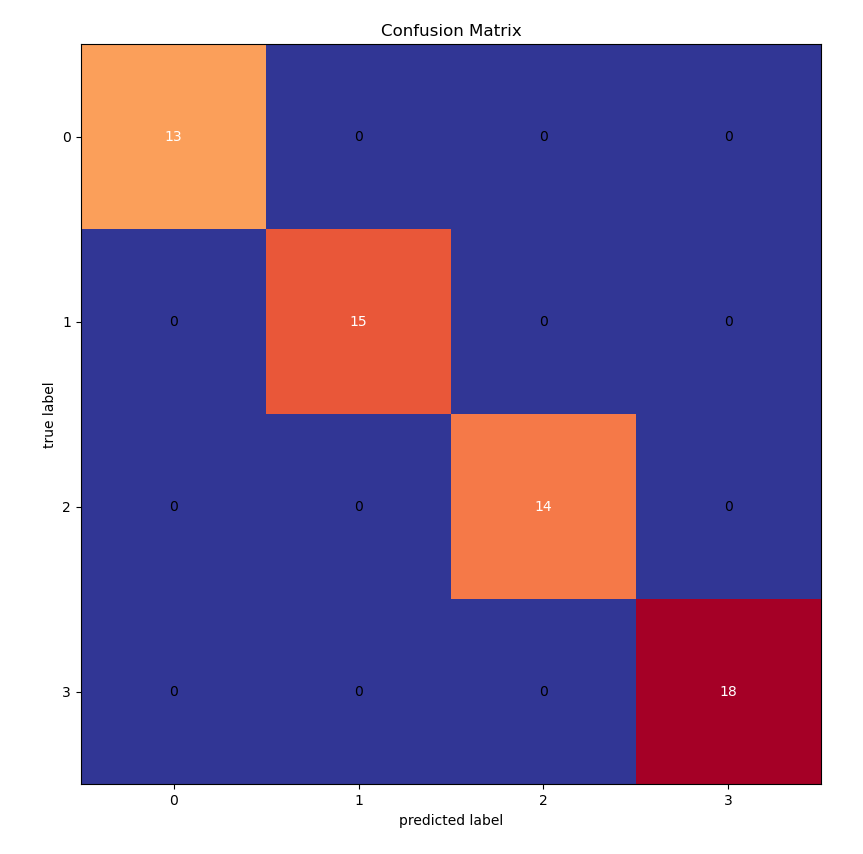
\includegraphics[height=2.3in]{Dataset_1a/K_15_cmatrix_test_data.png}
        \caption{Confusion Matrix for test data}
    \end{subfigure}%
    ~
    \caption{Confusion Matrix for KNN Model trained with K=15}
    \label{fig:5}
\end{figure}
% -----------------------------------------------------------
\begin{figure}[!ht]
    \centering
    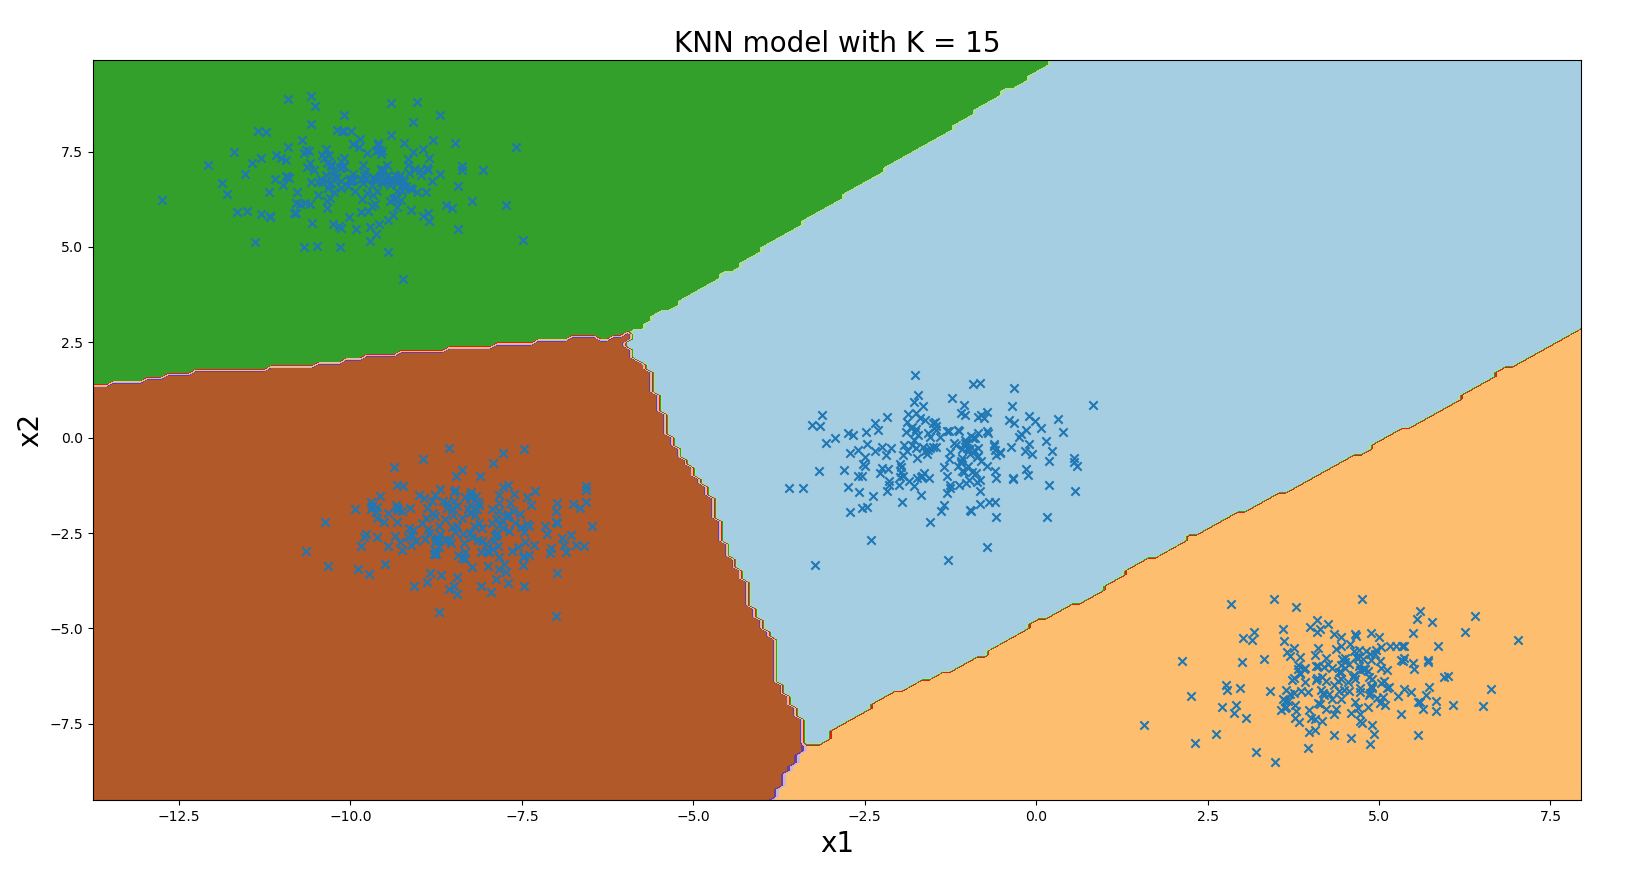
\includegraphics[height=3.5in,width=4in]{Dataset_1a/K_15_decision_plot.png}
    \caption{Decision Plot KNN Model trained with K=15}
    \label{fig:6}
\end{figure}

% -----------------------------------------------------------
\subsection{Naive Bayes Classifier with Gaussian Distribution}

The covariance matrix is a diagonal matrix in the case of naive bayes classifier and the nature of the matrix is experimented in this section to study about the various observations in the decision plot. Let us look at several interesting plots. \\

Similar to the case of KNN, the model accuracies didn't vary much in this case well since it is a synthetic data and we get very good results as can be observed from the confusion matrices and [\ref{table:2}]. The decision boundary in all the 3 cases are observed to be linear since we assume that the covariance matrix is diagonal. The level curves of the gaussian function assumed is a circle/ellipse with its axes parallel to the coordinate axes in all the 3 cases. Case 1: [\ref{fig:8}] has a circular level curve. All other cases have an elliptical level curve. Since the variance is very small, the elliptical nature is not directly visible from their plots. Here \textit{C1, C2} represent the covariance matrix for different classes. For the sake of convenience we only represent the conditions using 2 classes but in our case, we have 4 classes involved.

\hspace{5cm}
% ---------------------------------------------------------
{\rowcolors{3}{green!40!yellow!10}{green!0!yellow!30}
\begin{table}[!h]
\centering
\begin{tabular}{ |c|c|c| }
\hline
\rowcolor{lightgray} Model & Train Accuracy & Val Accuracy \\
\hline
$C1=C2=\sigma^2I$ & 100$\%$  & 100$\%$\\   
 \hline
$C1=C2$ & 100$\%$  & 100$\%$ \\ 
 \hline
$C1 \neq C2$ & 100$\%$  & 100$\%$\\ 
\hline
\end{tabular}
\caption{Performance of various Naive Bayes Models}.
\label{table:2}
\end{table}
}

\newpage
%-------------------------------------------------------------
\subsubsection{Plots for $C1=C2=\sigma^2I$}

\begin{figure}[!ht]
    \centering
    \begin{subfigure}[t]{0.5\textwidth}
        \centering
        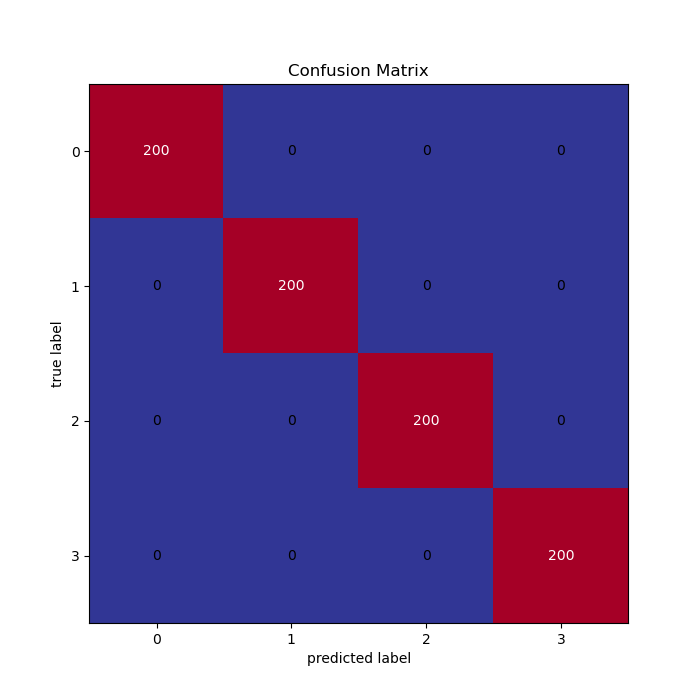
\includegraphics[height=2.5in]{Dataset_1a/Naive_Bayes_Classifier_case1_cmatrix_train_data.png}
        \caption{Confusion Matrix for training data}
    \end{subfigure}%
    ~ 
    \begin{subfigure}[t]{0.5\textwidth}
        \centering
        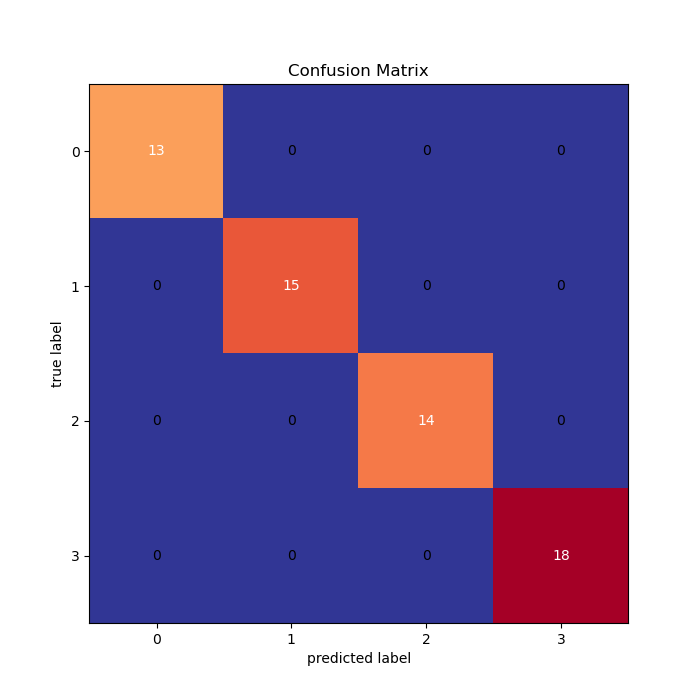
\includegraphics[height=2.5in]{Dataset_1a/Naive_Bayes_Classifier_case1_cmatrix_test_data.png}
        \caption{Confusion Matrix for test data}
    \end{subfigure}%
    ~
    \caption{Confusion Matrix for Naive Bayes Model trained with $C1=C2=\sigma^2I$}
    \label{fig:7}
\end{figure}

% ------------------------------------------------------------
\begin{figure}[!ht]
    \centering
    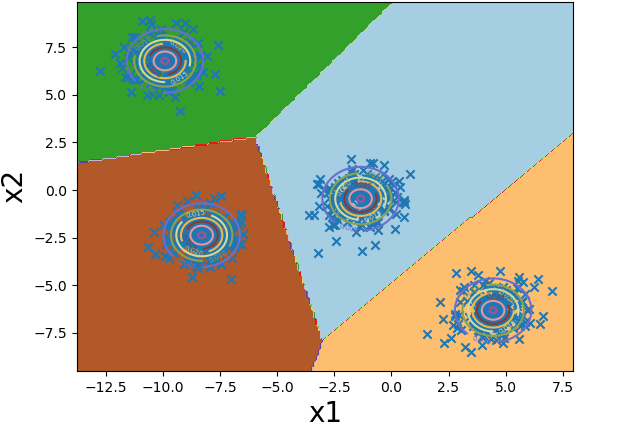
\includegraphics[height=3.5in]{Dataset_1a/Naive_Bayes_Classifier_case1_decision_plot.png}
    \caption{Decision Plot of Naive Bayes Model trained with $C1=C2=\sigma^2I$}
    \label{fig:8}
\end{figure}

\newpage
% ------------------------------------------------------------
\subsubsection{Plots for $C1=C2$ }

\begin{figure}[!ht]
    \centering
    \begin{subfigure}[t]{0.5\textwidth}
        \centering
        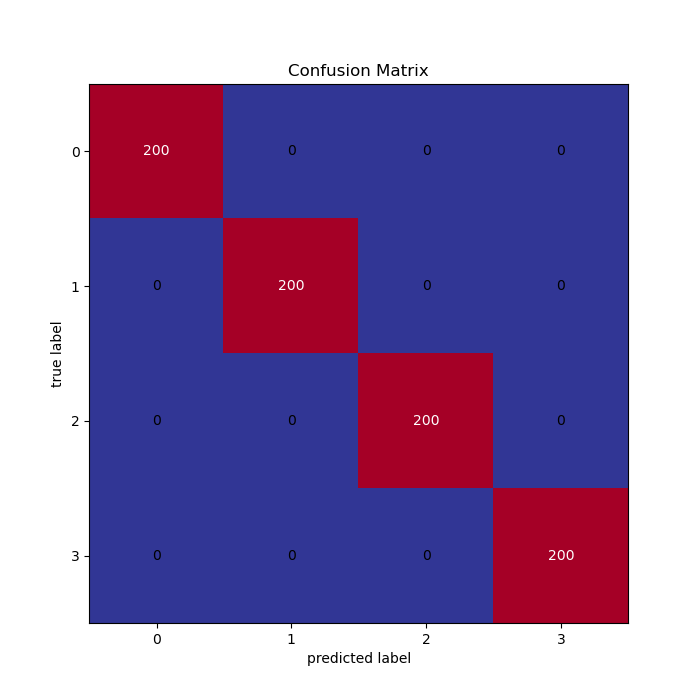
\includegraphics[height=2.5in]{Dataset_1a/Naive_Bayes_Classifier_case1_cmatrix_train_data.png}
        \caption{Confusion Matrix for training data}
    \end{subfigure}%
    ~ 
    \begin{subfigure}[t]{0.5\textwidth}
        \centering
        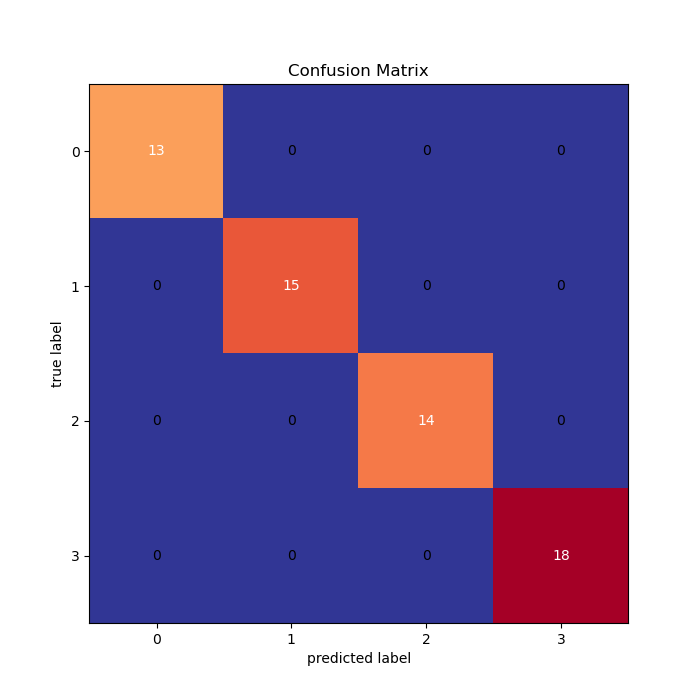
\includegraphics[height=2.5in]{Dataset_1a/Naive_Bayes_Classifier_case1_cmatrix_test_data.png}
        \caption{Confusion Matrix for test data}
    \end{subfigure}%
    ~
    \caption{Confusion Matrix for Naive Bayes Model trained with $C1=C2$}
    \label{fig:9}
\end{figure}

% ------------------------------------------------------------
\begin{figure}[!ht]
    \centering
    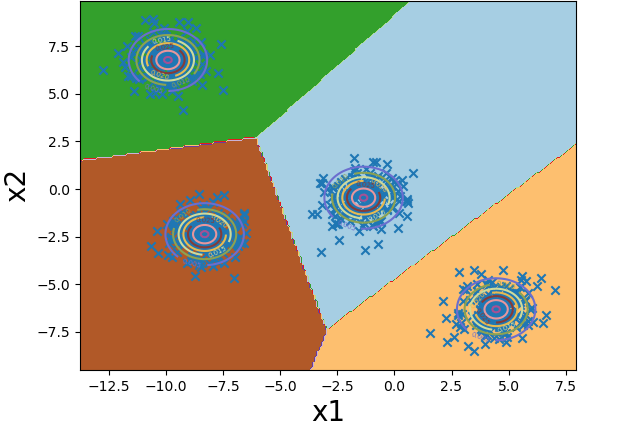
\includegraphics[height=3.5in]{Dataset_1a/Naive_Bayes_Classifier_case2_decision_plot.png}
    \caption{Decision Plot of Naive Bayes Model trained with $C1=C2$ }
    \label{fig:10}
\end{figure}

\newpage
% ------------------------------------------------------------
\subsubsection{Plots for $C1 \neq C2$ }

\begin{figure}[!ht]
    \centering
    \begin{subfigure}[t]{0.5\textwidth}
        \centering
        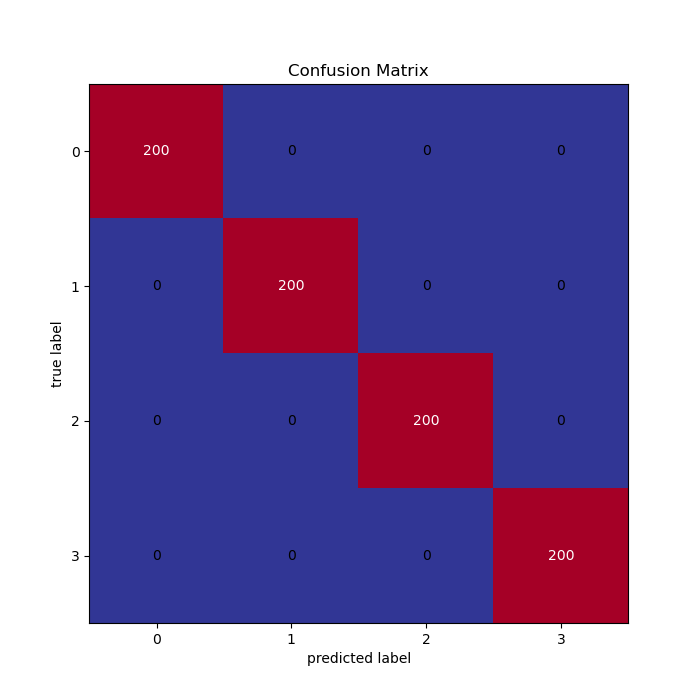
\includegraphics[height=2.5in]{Dataset_1a/Naive_Bayes_Classifier_case1_cmatrix_train_data.png}
        \caption{Confusion Matrix for training data}
    \end{subfigure}%
    ~ 
    \begin{subfigure}[t]{0.5\textwidth}
        \centering
        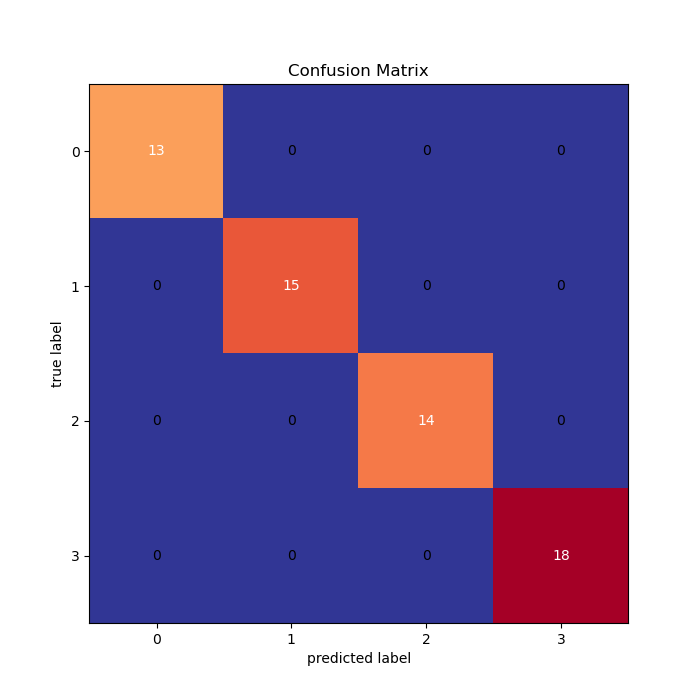
\includegraphics[height=2.5in]{Dataset_1a/Naive_Bayes_Classifier_case1_cmatrix_test_data.png}
        \caption{Confusion Matrix for test data}
    \end{subfigure}%
    ~
    \caption{Confusion Matrix for Naive Bayes Model trained with $C1 \neq C2$}
    \label{fig:11}
\end{figure}

% ------------------------------------------------------------
\begin{figure}[!ht]
    \centering
    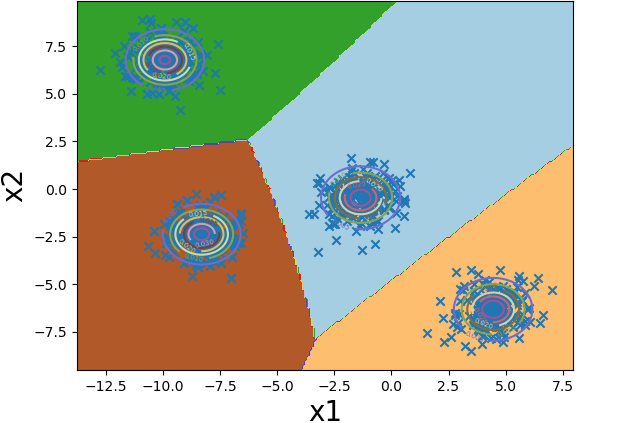
\includegraphics[height=3.3in]{Dataset_1a/Naive_Bayes_Classifier_case3_decision_plot.png}
    \caption{Decision Plot of Naive Bayes Model trained with $C1 \neq C2$ }
    \label{fig:12}
\end{figure}
% ----------------------------------------------------------



